\documentclass[12pt]{report}
\usepackage[spanish, activeacute]{babel}
\usepackage[top=2.75cm,bottom=2.50cm,left=3.00cm,right=2.50cm]{geometry}
\usepackage[utf8]{inputenc}  
\usepackage{enumerate}
\usepackage{graphicx}



\begin{document}

\setlength{\unitlength}{1 cm} %ESPOL
\thispagestyle{empty}
\begin{picture}(18,4)
\put(0,0){
\includegraphics[width=3cm,height=4cm]{imagenes_usuario/comicit.jpg}}
\put(11.5,0){
\includegraphics[width=4cm,height=4cm]{imagenes_usuario/comicit.jpg}}
\end{picture}
\\
\\
\begin{center}
\textbf{{\Huge Espol}\\[0.5cm]
{\LARGE Escuela Superior Politécnica del Litoral}}\\[1.25cm]
{\Large Lenguajes de Programación}\\[2.3cm]
{\LARGE \textbf{Manual de Usuario}}\\[3.5cm]
{\large Ana Arias}\\[2cm]
{\large Liliana Ramos}\\[2cm]
{\large Denny Schuldt}\\[2cm]
2º Ingeniería Ciencias Computacionales \\[1cm]
Ecuador - \today
\end{center}


	\setlength{\topmargin}{-0.5in}
	\pagestyle{empty}
	\begin{center}
		\textbf{
			\vspace{-0.7em}
			ESCUELA SUPERIOR POLITÉCNICA DEL LITORAL
		}
		\line(1,0){380}\\		
		\scriptsize{FACULTAD DE INGENIERÍA EN ELECTRICIDAD Y COMPUTACIÓN}
	\end{center}
	\begin{center}
		\vspace{2.5em}
		Lenguajes de Programación
		\\2012 | II Término
		\vspace{1.5em}
		\\Ana Arias - acarias@espol.edu.ec
		\vspace{4mm}
		\\Liliana Ramos - ljramos@espol.edu.ec
		\\Denny Schuldt - dschuldt@espol.edu.ec



\tableofcontents

\chapter{Introducción}
		\vspace{2em}
		\Huge{\textbf{\\Comic It!	\vspace{1em}}}
	\end{center}	

\begin{center}
		\begingroup
			
\includegraphics[width=0.30\textwidth]{imagenes_usuario/comicit.jpg}
		\endgroup
	\end{center}
	\begingroup
		\large{
			\textbf{
				INTRODUCCION
				\newline
				\newline
			}
		}
	\endgroup

	%
	%
	%
``Comic It!'' es una nueva aplicación para disposivos móviles que utilizan como sistema operativo Android. El nombre representa completamente a este nuevo software, puesto que será diseñado para crear historietas.
\newline
\newline
``Comic It!'' tendrá como usuarios a personas que les gusta tomar fotos y conservar recuerdos de los momentos divertidos que viven diariamente.
\newline
\newline
Con plantillas para colocar sus fotos, burbujas de diálogo e imágenes predeterminadas, el usuario quedará satisfecho cuando obtenga su obra final en su dispositivo.
\newline
\newline
Esta historieta relatará de una manera divertida, humorística y muy colorida exactamente lo que el usuario ha vivido o haya querido inventar para su uso personal.
	

Comic It! cuenta con una variedad de funcionalidades que el usuario puede usar de manera rápida y dinámica utilizando 				fotos tomadas directamente de la CÁMARA o de la GALERÍA FOTOGRÁFICA .
\newline
\newline
El usuario tendrá la opción de crear un collage tipo caricatura  con fotografías de la galería de fotos del celular en una plantilla escogida de una LISTA DE PLANTILLAS proporcionadas por la aplicación.
\newline
\newline
Comic It! cuenta con una LISTA DE ÍCONOS básicos y personalizados que permitirán al usuario crear imágenes más reales y divertidas.	
\newline
\newline	
Además de íconos, el usuario tendrá una LISTA DE TEXTOS divertidos para darle mas creatividad a las escenas que esté creando.
\newline
\newline
Proporciona una lista con varios formatos de BURBUJAS DE DIALOGO, de las cuales el usuario puede escoger las que más se ajuste a su necesidad. El usuario podrá EDITAR EL TEXTO dentro de la burbuja de dialogo que haya escogido, convirtiendo a los miembros de 		la fotografía en auténticos personajes.
\newline
\newline
Al terminar de crear caricaturas, se podrán guardar en la galería fotográfica en distintos FORMATOS.


%--------------------------------------------------------------------------------------------------------------------
\newpage
\chapter{Manual de usuario}

Espere mientras la aplicación ComicIt! es cargada completamente.


	\begin{center}
		\begingroup
			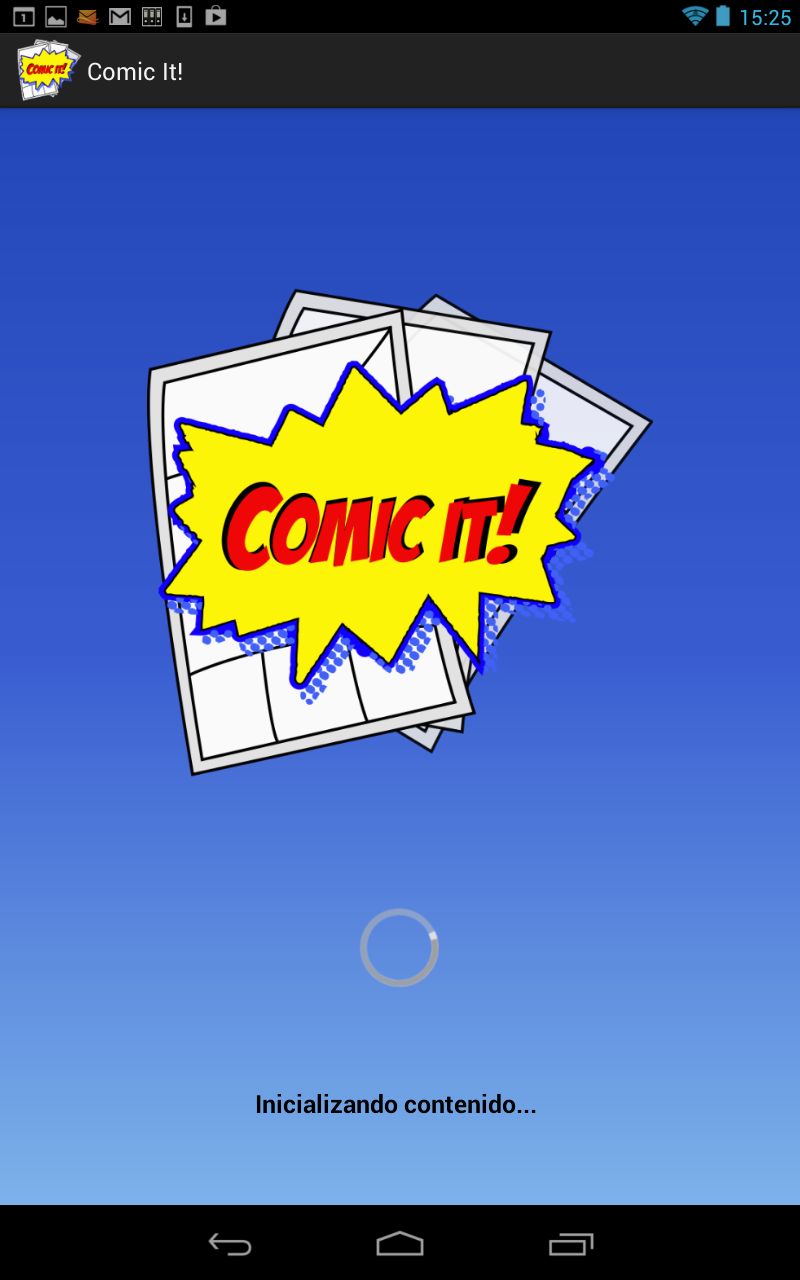
\includegraphics[width=0.30\textwidth]{imagenes_usuario/cargar.png}
		\endgroup
	\end{center}

Al abrir la aplicación se encontrarán las opciones de plantillas, de las cuales el usuario puede escoger la que desee según el tipo de caricatura que desee crear; estas plantillas contienen la opción de colocar 5 imágenes, colocadas en distintas posiciones según el diseño de la plantilla.

	\begin{center}
		\begingroup
			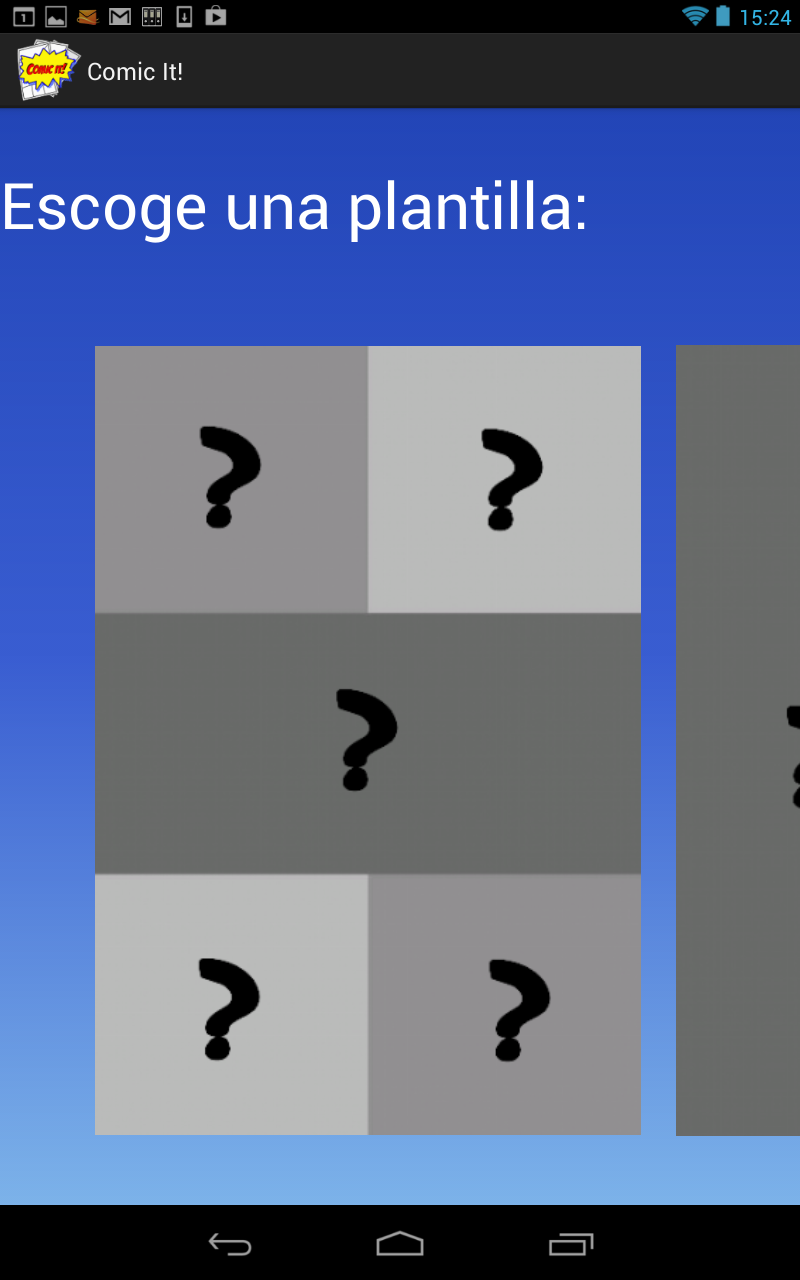
\includegraphics[width=0.32\textwidth]{imagenes_usuario/plantillas.png}
		\endgroup
	\end{center}


Al darle un click a la plantilla que se desea escoger se abrirá una ventana en la cual la plantilla escogida saldrá en toda la pantalla. El usuario podrá empezar a crear su caricatura!
Para poder colocar fotos en los recuadros de la plantilla, el usuario tendrá que darle click al recuadro que desea rellenar con fotos tomadas ya sea desde la cámara o la galería de fotos del celular
\newline

	\begin{center}
		\begingroup
			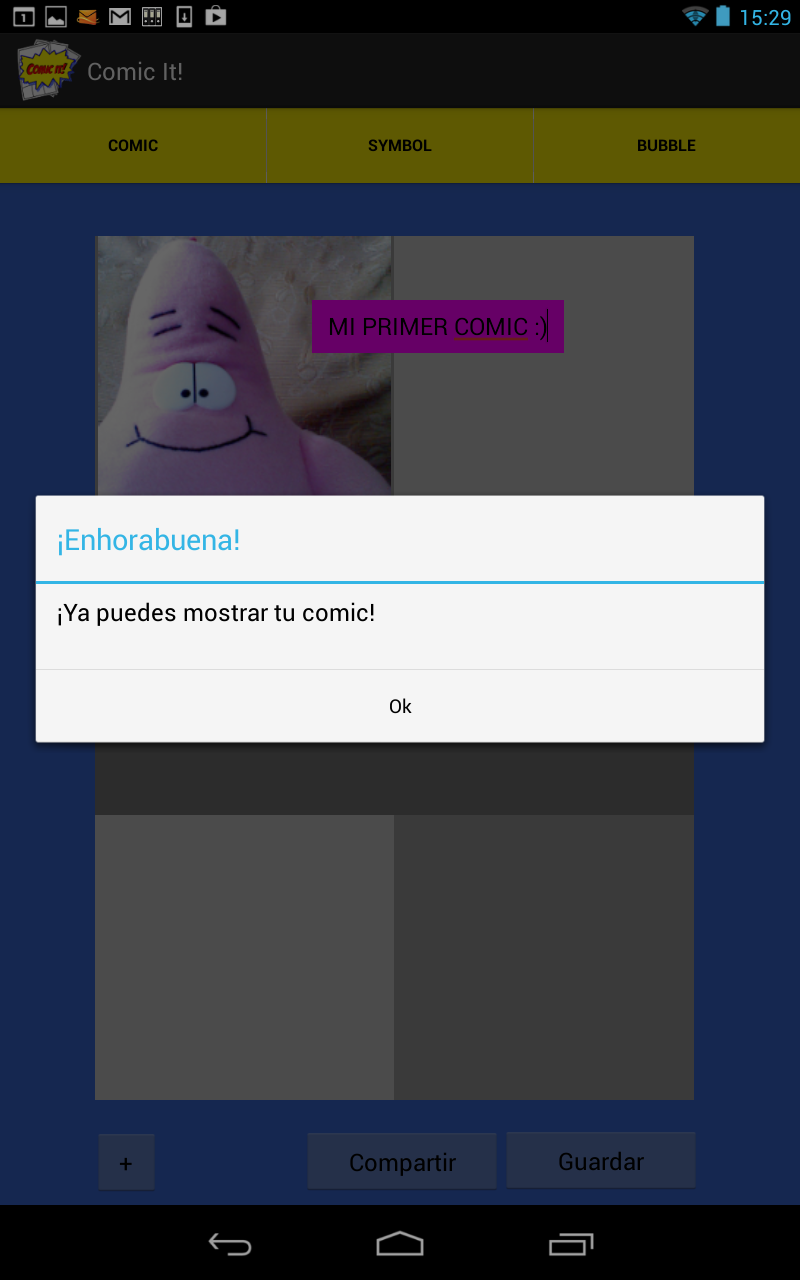
\includegraphics[width=0.33\textwidth]{imagenes_usuario/camara.png}
		\endgroup
	\end{center}

Si se escoge la opción cámara, automáticamente aparecerá la cámara del celular, de la cual se tomará la foto deseada.
\newline
	\begin{center}
		\begingroup
			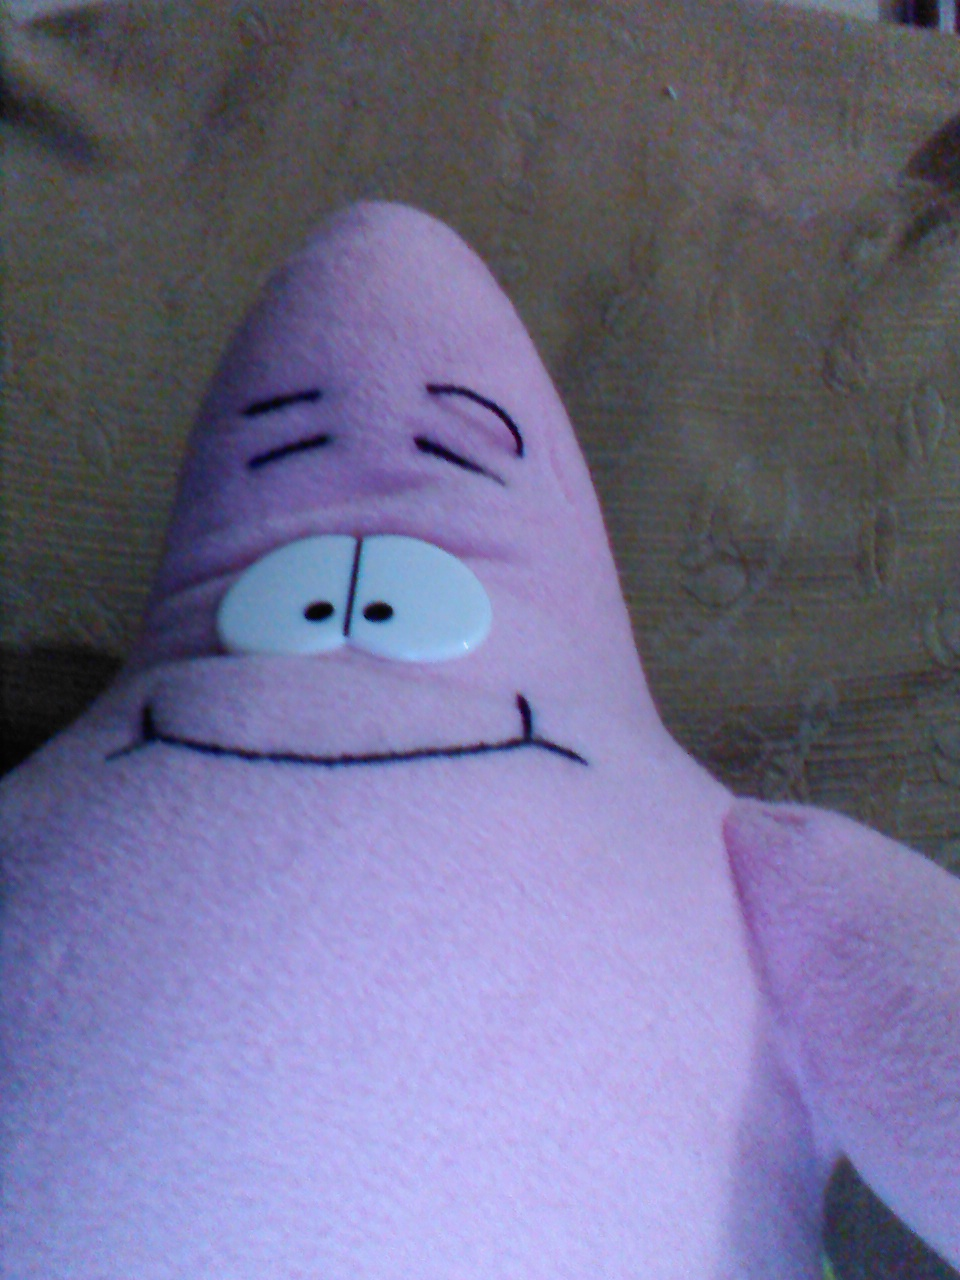
\includegraphics[width=0.40\textwidth]{imagenes_usuario/foto.jpg}
		\endgroup
	\end{center}



Si por el contrario se escoge la galería de fotos, se abrirá automáticamente la galería fotográfica del celular, en la que se deberá buscar la foto deseada y escogerla.
\newline
	\begin{center}
		\begingroup
			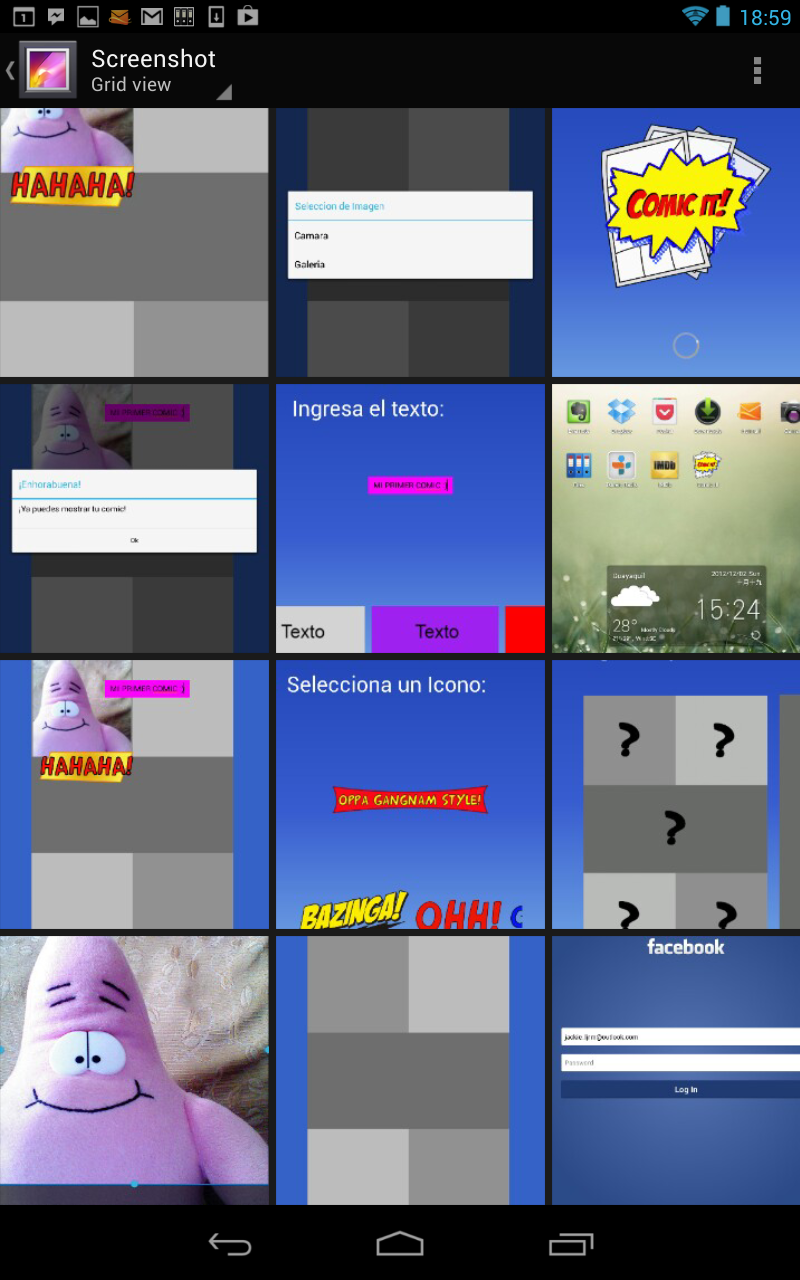
\includegraphics[width=0.33\textwidth]{imagenes_usuario/galeria.png}
		\endgroup
	\end{center}


Una vez obtenida la foto deseada, se creará automáticamente la opción para recortar dicha foto, y así determinar el rango de imagen que se desea de la foto tomada.
\newline
	\begin{center}
		\begingroup
			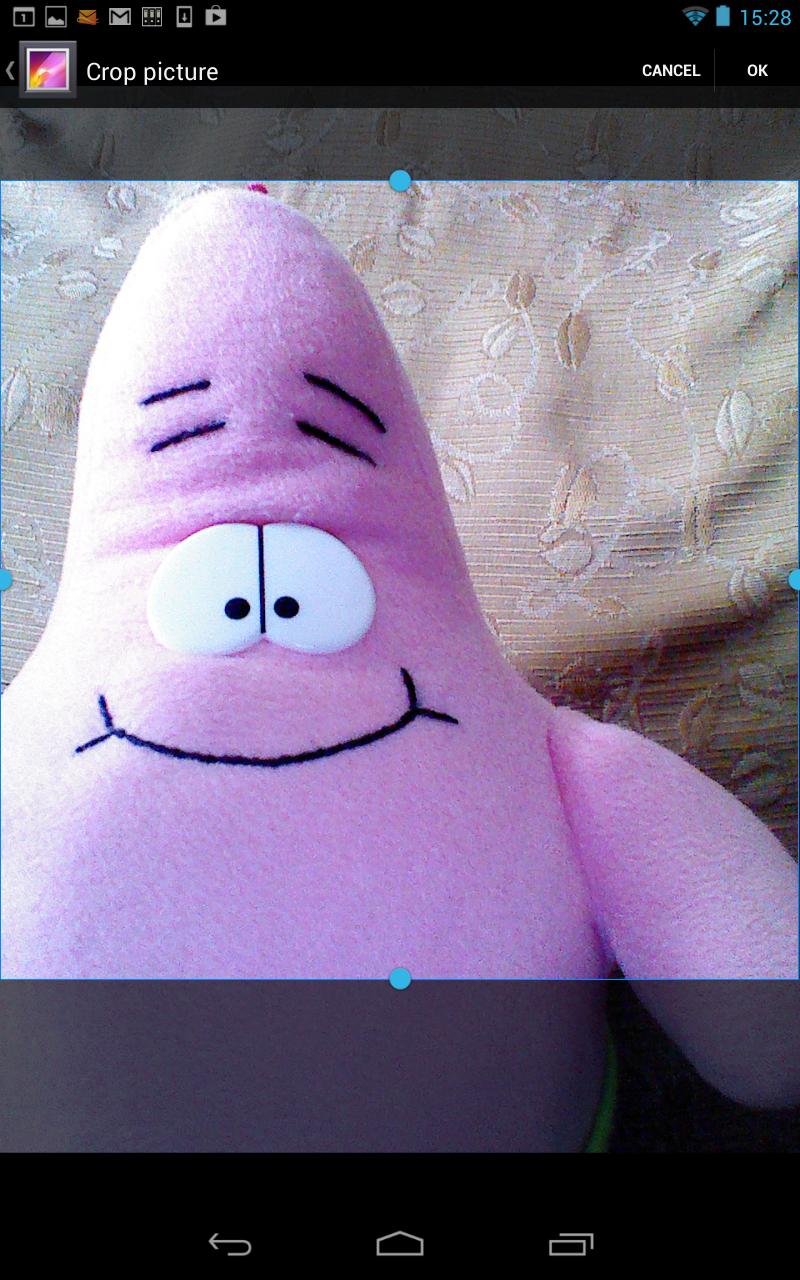
\includegraphics[width=0.33\textwidth]{imagenes_usuario/crop.png}
		\endgroup
	\end{center}

Luego de recortar la imagen y aceptar, la imagen obtenida y recortada se colocará en el recuadro que escogimos. Se debe repetir el proceso para los demás recuadros en la plantilla.
\newline
	\begin{center}
		\begingroup
			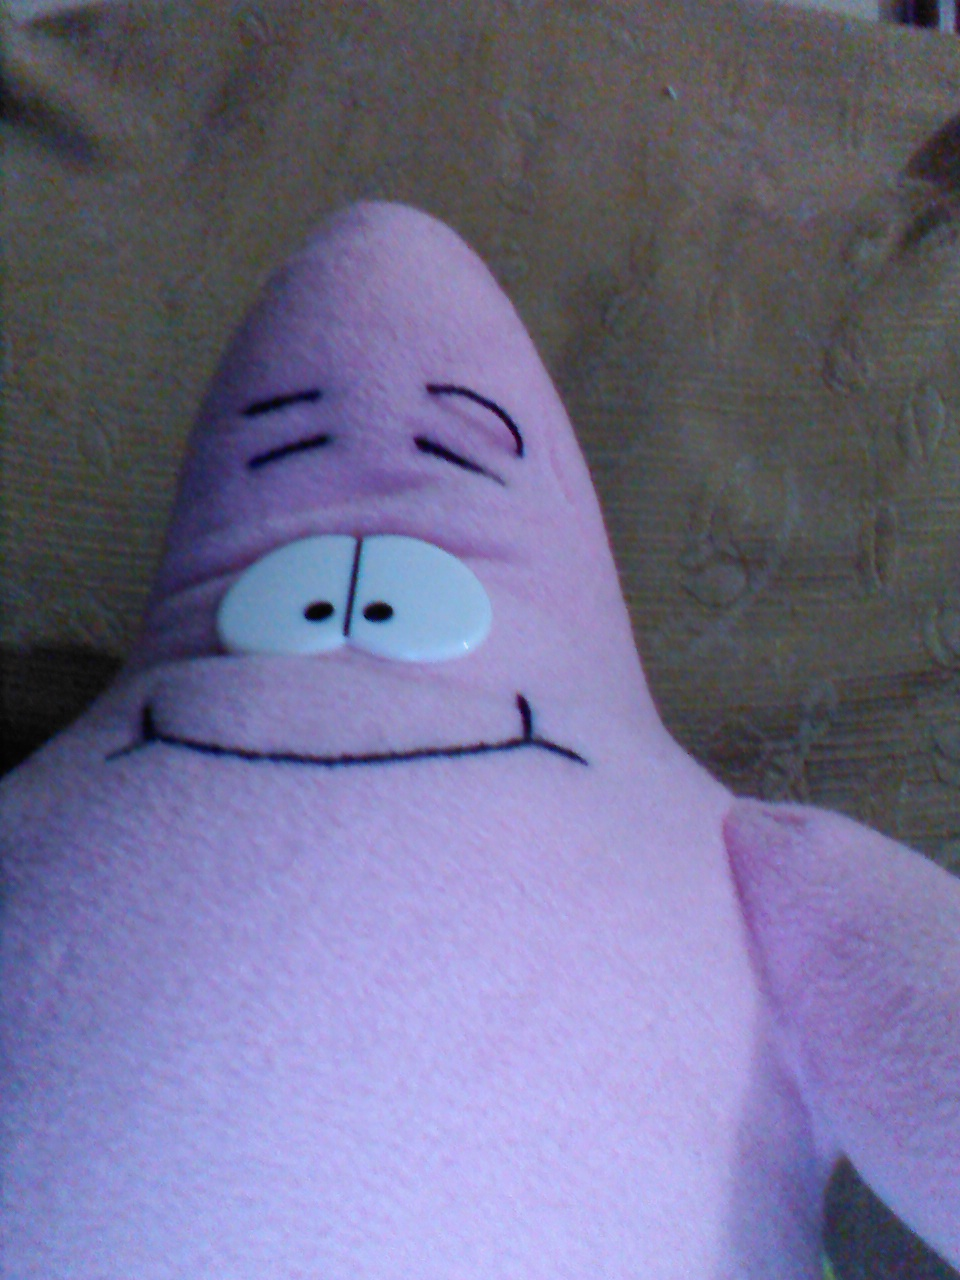
\includegraphics[width=0.33\textwidth]{imagenes_usuario/foto.jpg}
		\endgroup
	\end{center}


El usuario tiene la opción de cambiar la foto de los recuadros cuantas veces desee.
La plantilla está lista para convertirse en una caricatura.
El usuario tendrá las opciones de agregar a su plantilla, íconos con textos divertidos  y con diseños propios de los autores de Comic It!
Al escoger la opción de Symbols en los Tabs superiores, se abrirá una ventana que muestre la variedad de símbolos que el usuario puede escoger según lo que más se ajuste al tipo de caricatura que esté creando. Una vez escogido el símbolo, éste aparecerá en la plantilla que contiene las fotos anteriormente escogidas.
\newline

	\begin{center}
		\begingroup
			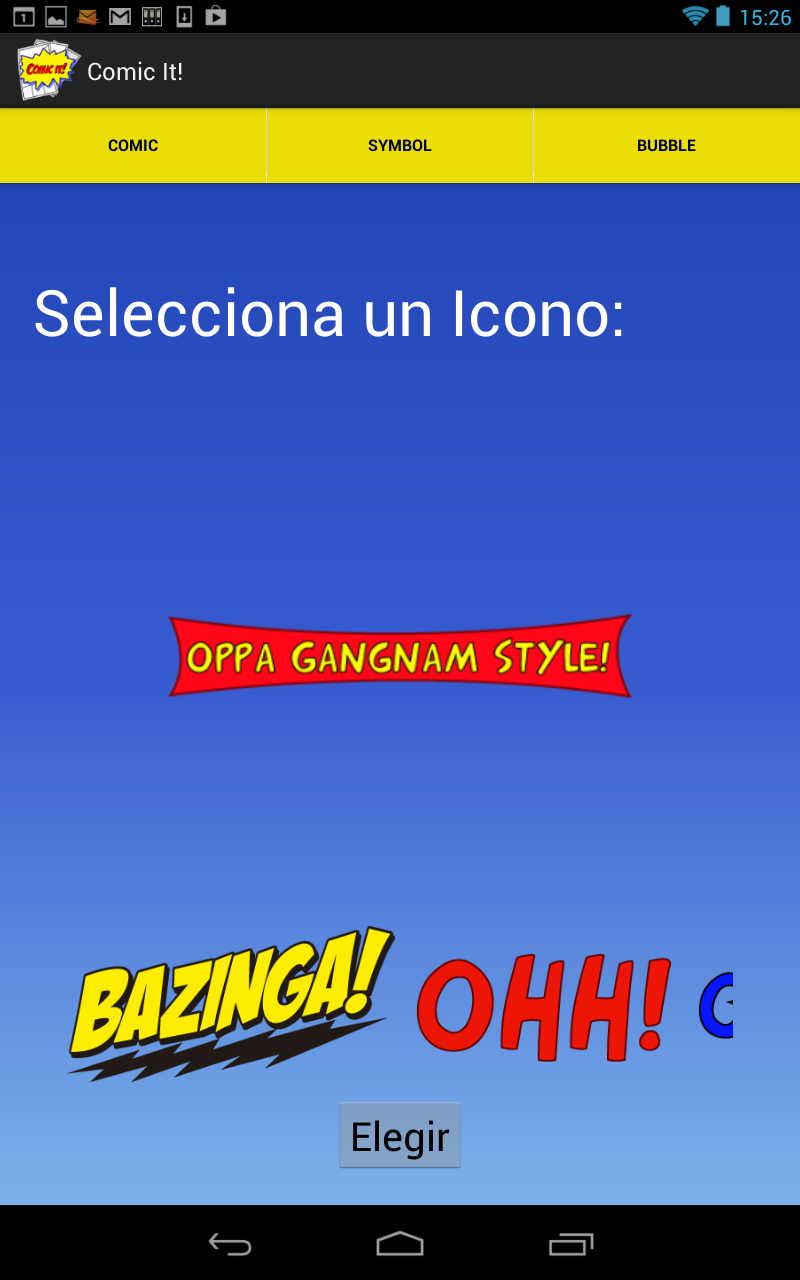
\includegraphics[width=0.33\textwidth]{imagenes_usuario/iconos.png}
		\endgroup
	\end{center}


El usuario tendrá la opción de arrastrar el ícono escogido en cualquier espacio de la plantilla. Podrá repetir el proceso con el número de íconos que desee colocar en su caricatura.
Al escoger la opción de Burbujas en los Tabs superiores, se abrirá una ventana que muestre la variedad de colores de burbujas que el usuario puede escoger según lo que más se ajuste al tipo de caricatura que esté creando. Una vez escogido el color de la burbuja, el usuario podrá escribir el texto que desee que esté en el interior de dicha burbuja; al terminar este proceso, la burbuja editada (con su correspondiente texto y color) aparecerá en la plantilla que contiene las fotos anteriormente escogidas.

	\begin{center}
		\begingroup
			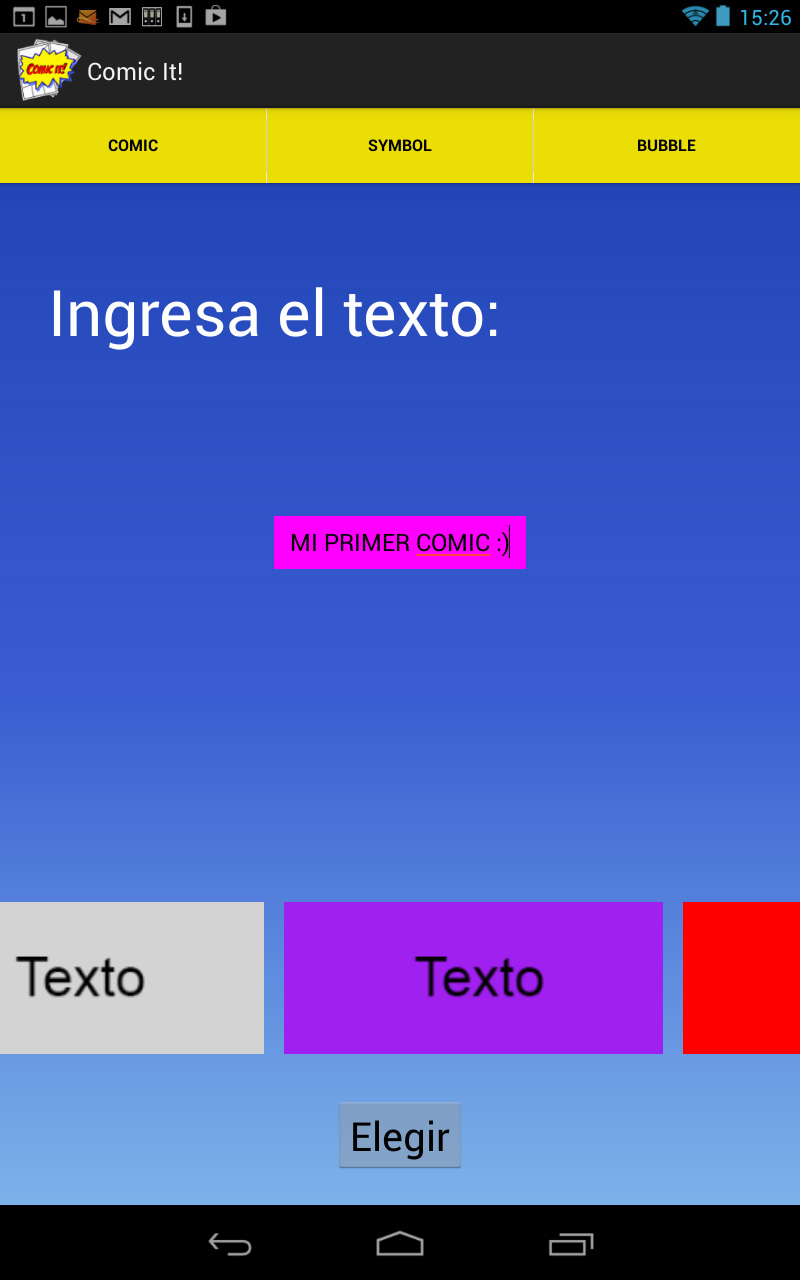
\includegraphics[width=0.30\textwidth]{imagenes_usuario/texto.png}
		\endgroup
	\end{center}

%--------------------------------------------------------------------------------------------------------------------


El usuario tendrá la opción de arrastrar la burbuja escogida en cualquier espacio de la plantilla. Podrá repetir el proceso con el número de burbujas que desee colocar en su caricatura.


	\begin{center}
		\begingroup
			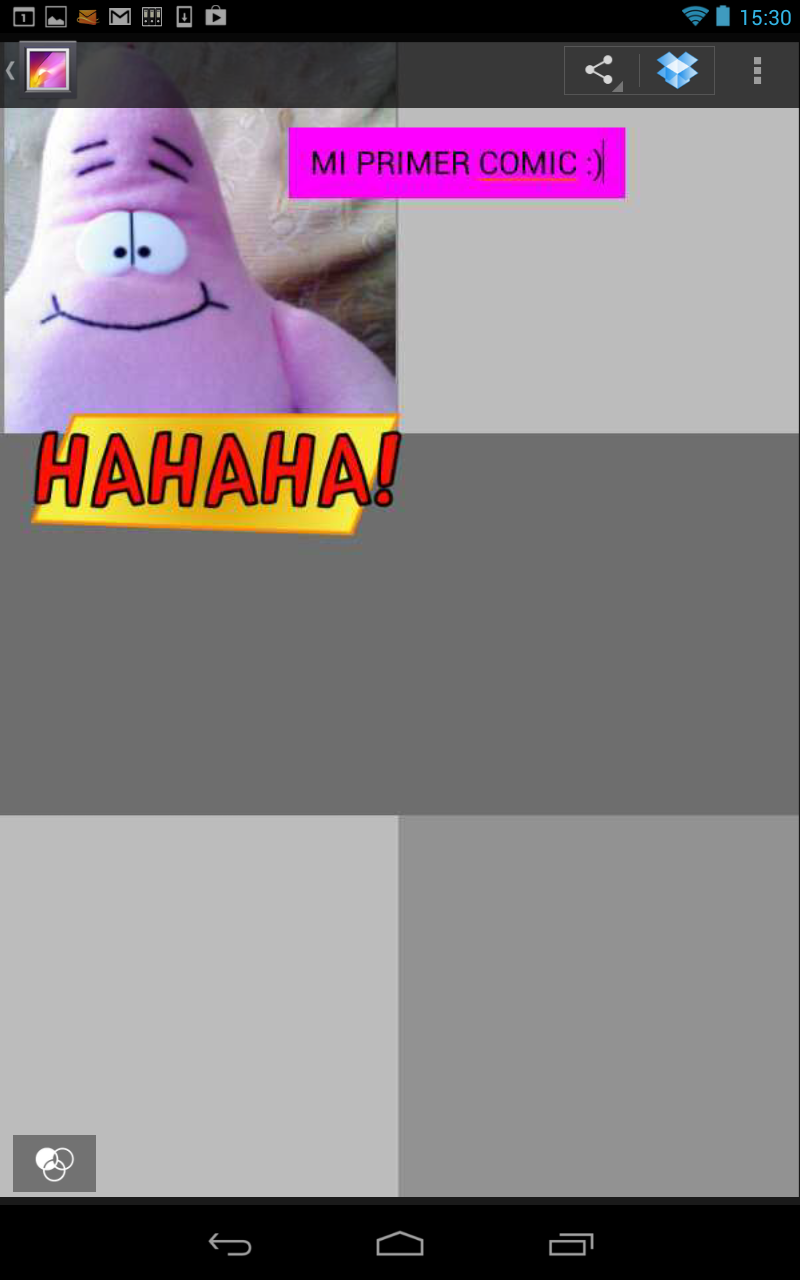
\includegraphics[width=0.30\textwidth]{imagenes_usuario/comic.png}
		\endgroup
	\end{center}

%--------------------------------------------------------------------------------------------------------------------
Presionar el botón guardar para que la caricatura se guarde en la memoria del celular.
Hoy en día las redes sociales son muy utilizadas en cualquier actividad que realicemos. ¿Por qué no compartir nuestra experiencia con amigos o familiares?
Por esto Comic It! permite compartir tu experiencia en Facebook.

	\begin{center}
		\begingroup
			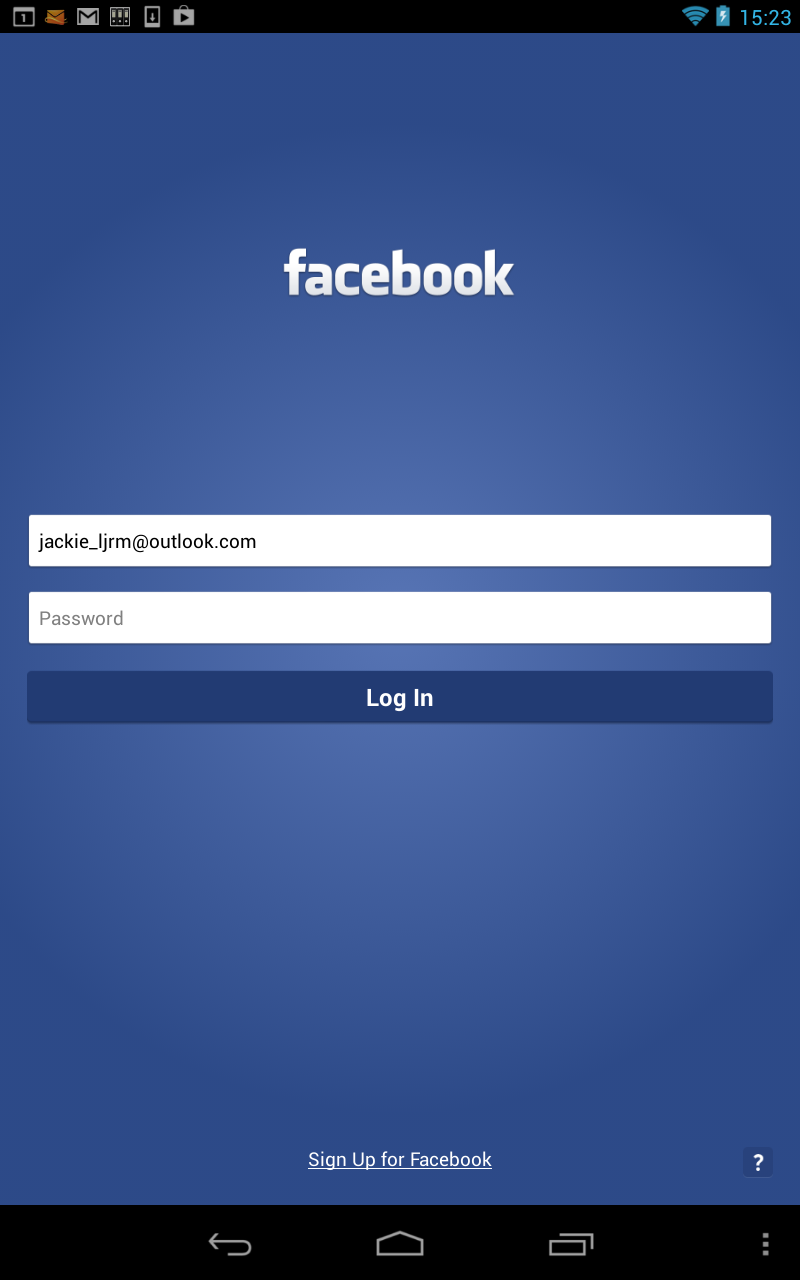
\includegraphics[width=0.33\textwidth]{imagenes_usuario/face.png}
		\endgroup
	\end{center}



\end{document}
